\documentclass[11pt]{article}
\usepackage[margin=1in]{geometry}
\usepackage{amsmath,amssymb,graphicx,listings,xcolor,float}

\lstset{
  language=Matlab,
  basicstyle=\small\ttfamily,
  keywordstyle=\color{blue},
  commentstyle=\color{green!50!black},
  stringstyle=\color{red},
  numbers=left,
  numberstyle=\tiny\color{gray},
  breaklines=true,
  frame=single,
  tabsize=4
}

\title{MATH 543 --- Homework 4\\Implement Modified Gram--Schmidt QR-Factorization}
\author{Parham Khodadi}
\date{}

\begin{document}
\maketitle

%% ============================================================
\section*{1. Modified Gram--Schmidt (MGS) Function}
%% ============================================================

Implemented \texttt{qr\_mgs(A)} following Algorithm 8.1 (p.58 of Trefethen \& Bau). See the MATLAB code in the Appendix.

%% ============================================================
\section*{2. Experiments \#1 and \#2}
%% ============================================================

\subsection*{Experiment \#1 (Figure 7.1)}

All three functions (MATLAB's \texttt{qr}, my CGS, and my MGS) reproduce Figure 7.1.

\begin{figure}[H]
\centering
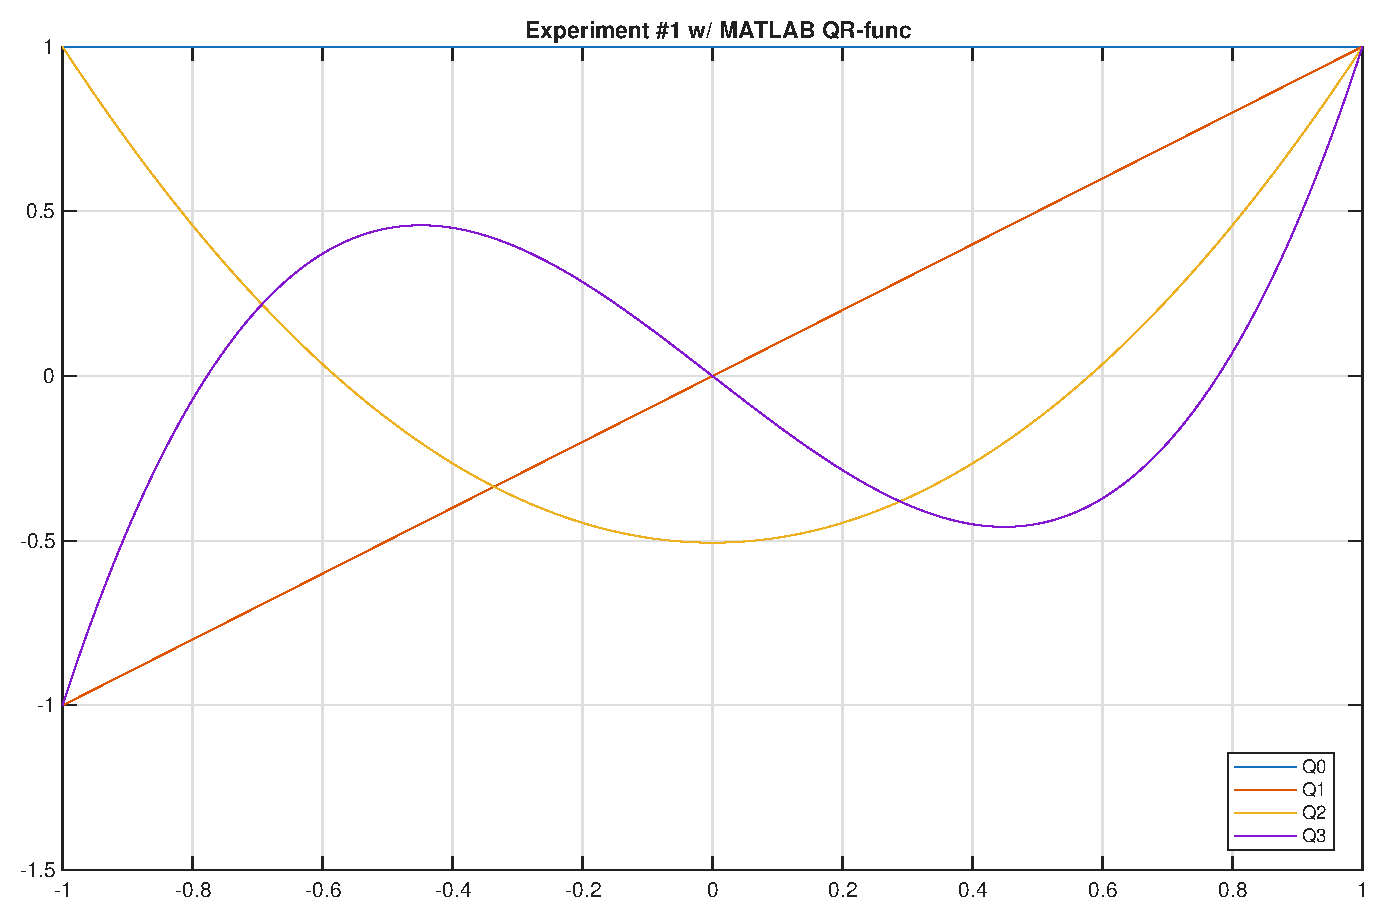
\includegraphics[width=\linewidth]{Figures/E1_QR.eps}
\caption{Experiment \#1 --- MATLAB's built-in QR.}
\end{figure}

\begin{figure}[H]
\centering
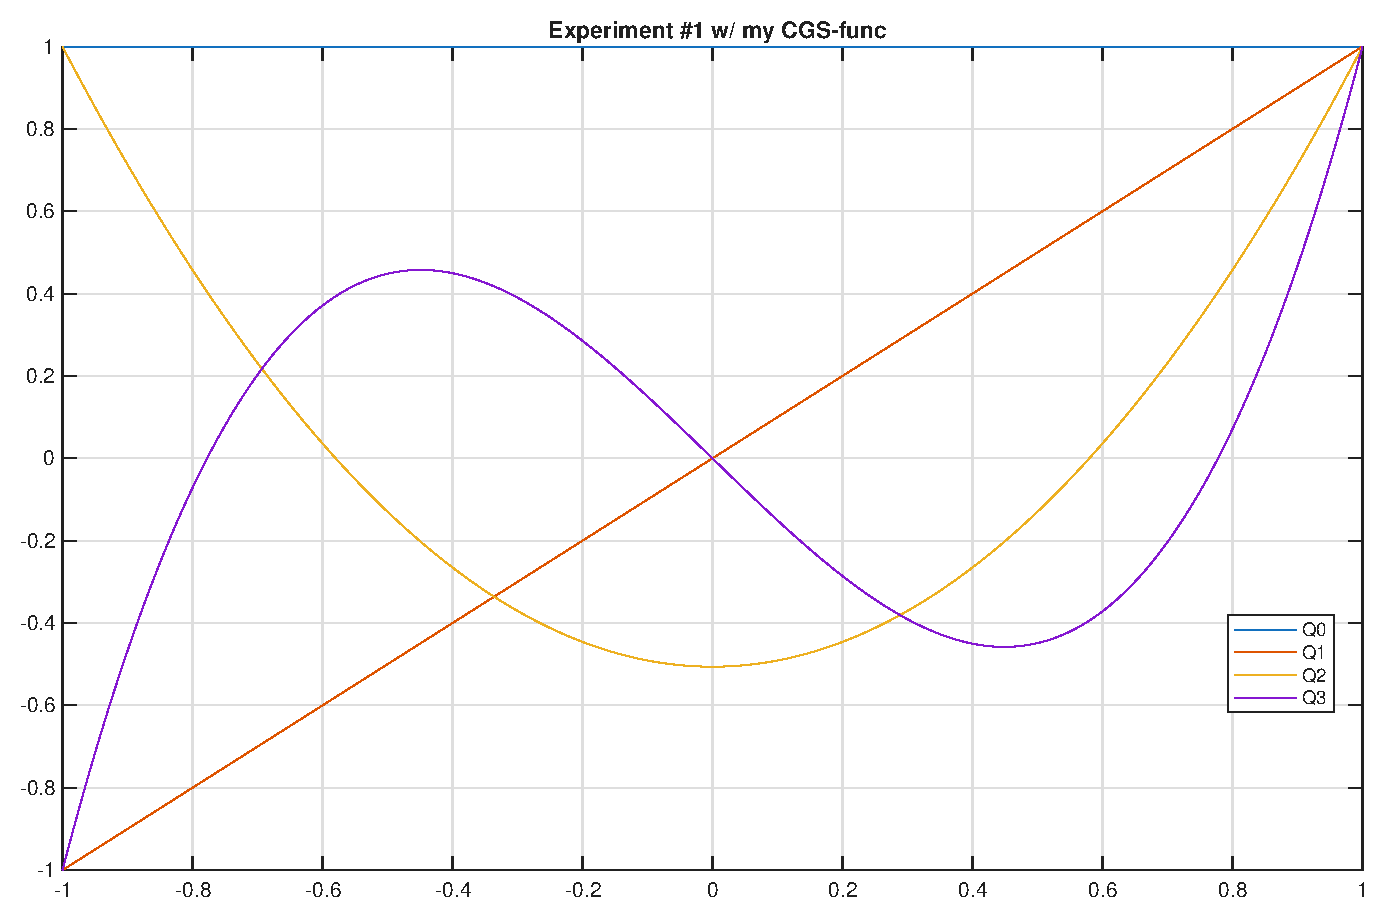
\includegraphics[width=\linewidth]{Figures/E1_CGS.eps}
\caption{Experiment \#1 --- Classical Gram--Schmidt.}
\end{figure}

\begin{figure}[H]
\centering
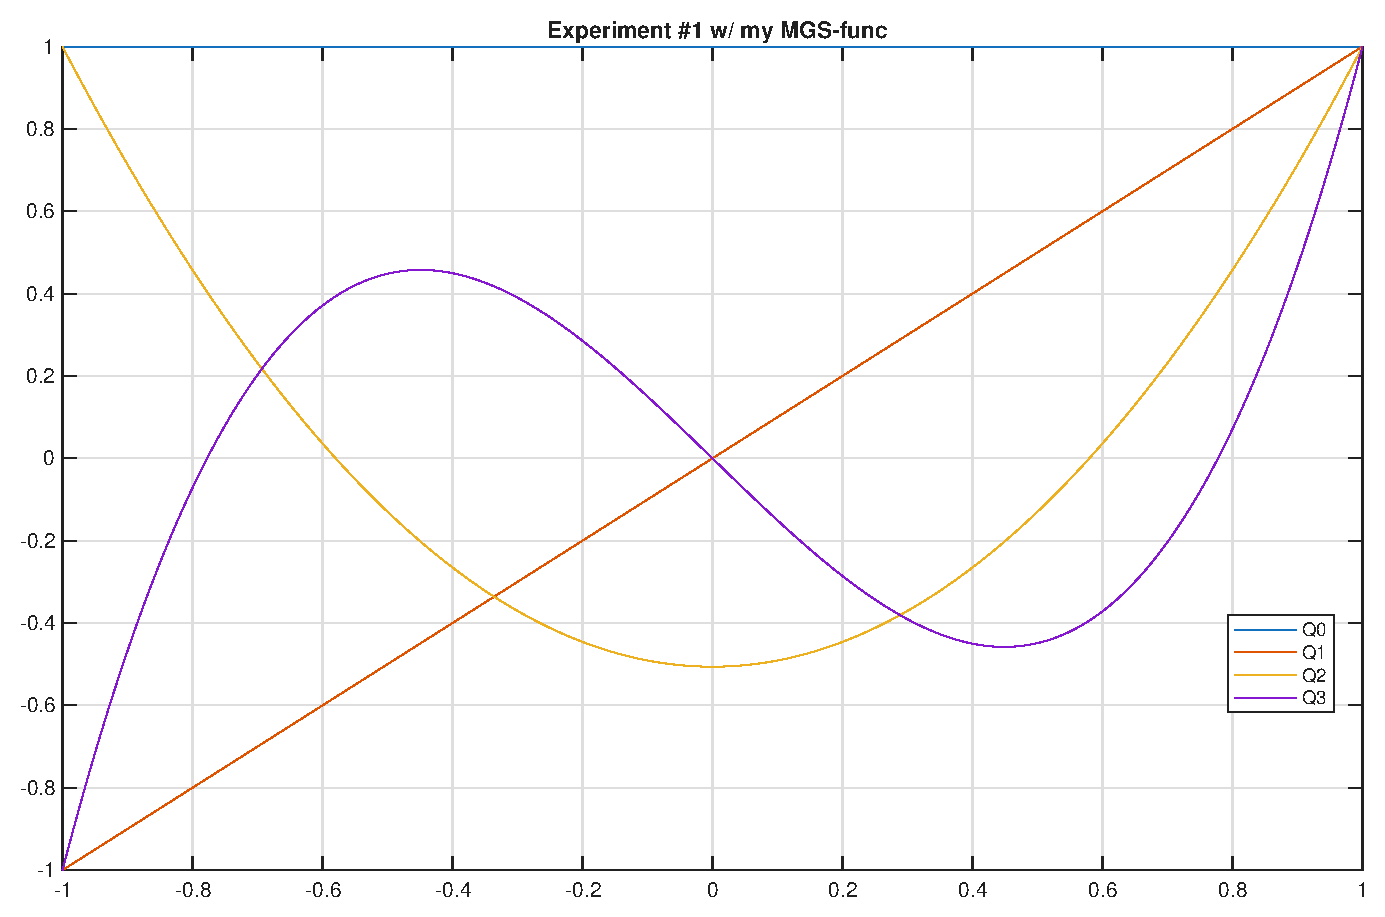
\includegraphics[width=\linewidth]{Figures/E1_MGS.eps}
\caption{Experiment \#1 --- Modified Gram--Schmidt.}
\end{figure}

\subsection*{Experiment \#2}

A matrix $A=U\Sigma V$ with $\sigma_j=2^{-j}$ is factored by CGS and MGS. The plot below shows $|r_{jj}|$ vs.\ $j$. CGS loses accuracy around $\sqrt{\epsilon_{\mathrm{machine}}}$, while MGS tracks $2^{-j}$ all the way down to $\epsilon_{\mathrm{machine}}$.

\begin{figure}[H]
\centering
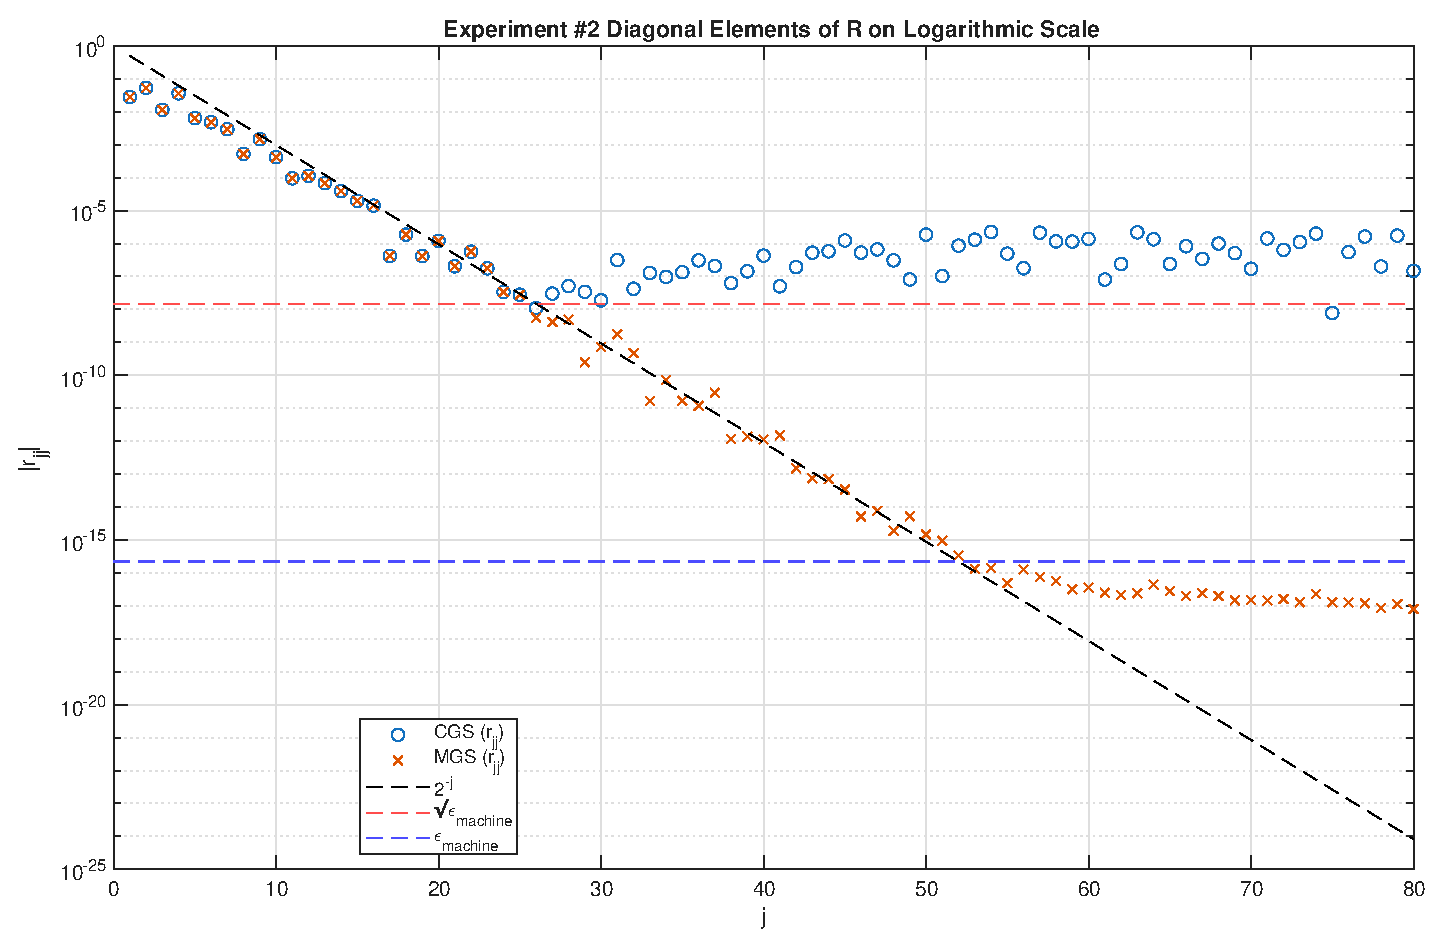
\includegraphics[width=\linewidth]{Figures/E2.eps}
\caption{Experiment \#2 --- Diagonal entries of $R$.}
\end{figure}

%% ============================================================
\section*{3. Exercise 9.1}
%% ============================================================

\subsection*{(a) Reproduce Figure 7.1}

Covered by Experiment \#1 above.

\subsection*{(b) Error vs.\ exact Legendre polynomials}

On the 257-point grid ($\Delta x=2^{-7}$), the MGS-computed $\tilde{P}_k$ are compared with the exact Legendre polynomials $P_0,\dots,P_3$. Maximum errors are $O(10^{-3})$--$O(10^{-2})$.

\begin{figure}[H]
\centering
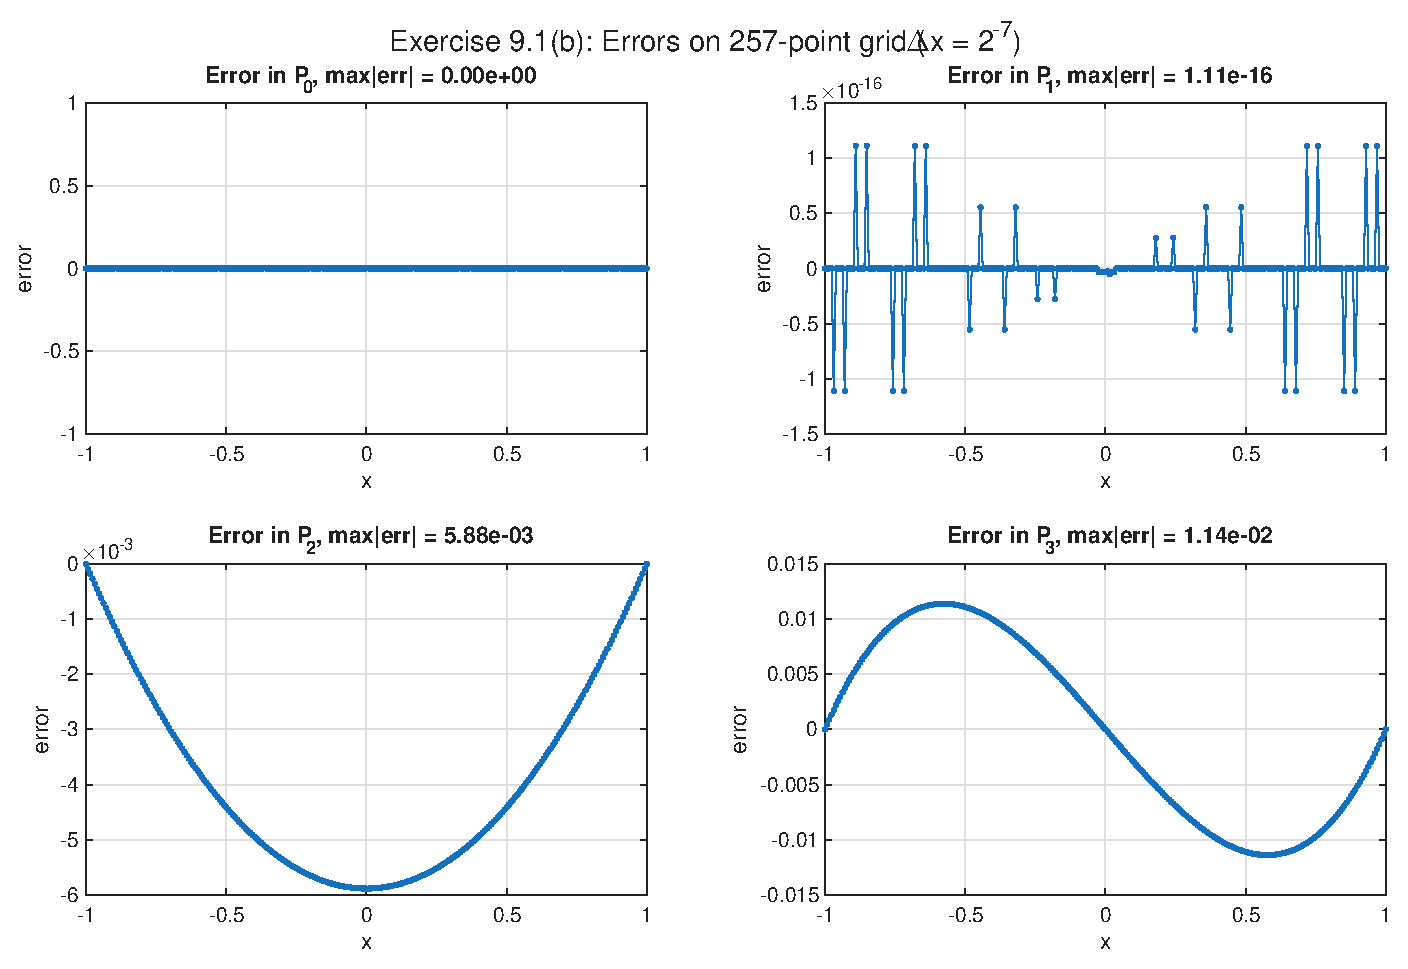
\includegraphics[width=\linewidth]{Figures/9_1_b.eps}
\caption{Exercise 9.1(b) --- Pointwise error on the 257-point grid.}
\end{figure}

\subsection*{(c) Convergence as $\Delta x\to 0$}

The grid is refined from $\nu=2$ to $\nu=10$ ($\Delta x=2^{-\nu}$). The semilogy plot below shows max error vs.\ $\nu$.

\begin{figure}[H]
\centering
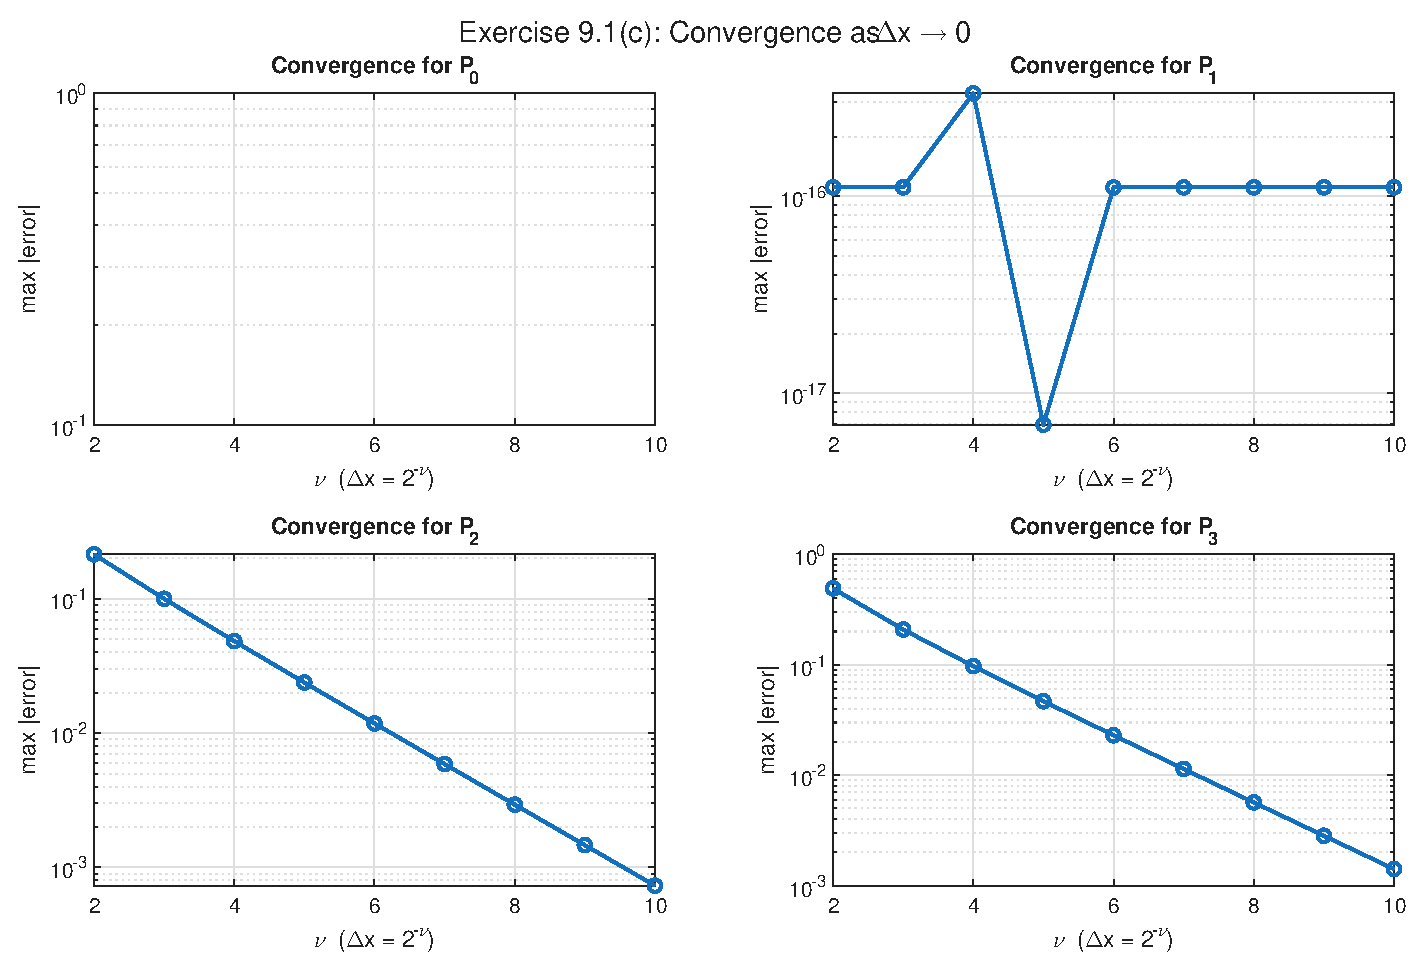
\includegraphics[width=\linewidth]{Figures/9_1_c.eps}
\caption{Exercise 9.1(c) --- Convergence as $\Delta x\to 0$.}
\end{figure}

% TODO: fill in your discussion of convergence rate here
From the plots, the error in $P_k$ decreases roughly as $(\Delta x)^{p}$ where:
\begin{itemize}
  \item $P_0$: exact (machine precision), so no meaningful power.
  \item $P_1$: exact (machine precision), so no meaningful power.
  \item $P_2$: the slope suggests $p\approx 2$.
  \item $P_3$: the slope suggests $p\approx 2$.
\end{itemize}
\textit{(Adjust the above after inspecting your plots.)}

%% ============================================================
\section*{4. Exercise 9.2}
%% ============================================================

Let $A=I+2N$ where $N$ is the $20\times20$ superdiagonal matrix of ones.

\subsection*{(a) Eigenvalues, determinant, rank}

All eigenvalues equal 1, $\det(A)=1$, and $\operatorname{rank}(A)=20$.

\subsection*{(b) Inverse}

$A^{-1}$ has entries that grow exponentially. Top-right $5\times5$ corner:
\[
\begin{pmatrix}
-32768 & 65536 & -131072 & 262144 & -524288\\
16384 & -32768 & 65536 & -131072 & 262144\\
-8192 & 16384 & -32768 & 65536 & -131072\\
4096 & -8192 & 16384 & -32768 & 65536\\
-2048 & 4096 & -8192 & 16384 & -32768
\end{pmatrix}
\]
The $(i,j)$ entry of $A^{-1}$ is $(-2)^{j-i}$ for $j\ge i$, and $0$ otherwise.

\subsection*{(c) Singular values}

\[
\sigma_{20} = 1.4305\times10^{-6},\qquad
\text{upper bound } \sqrt{\tfrac{3}{4^{20}-1}} = 1.6518\times10^{-6}.
\]
The bound holds: $\sigma_{20}\le\sqrt{3/(4^m-1)}$.

%% ============================================================
\newpage
\section*{Appendix: MATLAB Code}
%% ============================================================

\lstinputlisting{HW4.m}

\end{document}